% Lecture for ph2a Caltech 2017: Vibrations and Waves
\documentclass[pdf, handout, hideothersubsections]{beamer}
\usepackage{beamerthemeshadow}
\mode<presentation>
  {
    \usefonttheme{structuresmallcapsserif}
    \usetheme{CambridgeUS}
    \usecolortheme{seahorse}
    %\useinnertheme{circles}
%    \useoutertheme{tree}
  }

\usepackage{svg}
\usepackage{xmpmulti}
\usepackage{mathtools}
%\usepackage{enumitem}
\usepackage{hyperref}
\hypersetup{
    pdffitwindow=true,     % window fit to page when opened
    colorlinks=true,       % false: boxed links; true: colored links
    linkcolor=orange,      % color of internal links 
    citecolor=green,       % color of links to bibliography
    filecolor=magenta,     % color of file links
    urlcolor=blue,         % color of external links
    pdfstartview={Fit}
}

% Fonts/encoding
\renewcommand{\UrlFont}{\tiny}
\usepackage[utf8]{inputenc}
\usepackage[T1]{fontenc}
%\usepackage[sc,medium,raggedright]{titlesec}
\usepackage{newtxmath}
%\usepackage{libertine}
\usepackage[osf]{ebgaramond}

\graphicspath{{Figures/}}

\begin{document}
\title{Waving Strings}  
\author{Caltech: ph2a}
\date{17 - Oct - 2017}


\frame{\titlepage} 

\frame{\frametitle{Table of Contents}\tableofcontents} 

\setbeamerfont{footnote}{size=\tiny}

\section{Summary}
\begin{frame}
\frametitle{Last Time:}
\begin{itemize}
\item Coupled oscillators have multiple free vibration frequencies/modes.
\item These free oscillation frequencies are called eigenfrequencies.
\item The oscillation functions are the eigenfunctions.
\item Linear algebra can be used to solve for these functions.
\end{itemize}
\end{frame}


\begin{frame}
\frametitle{Overview}
\begin{enumerate}
  \pause
\item Matrix methods can be used to analyzed eigenmodes of linear systems.
  \pause
\item The case of $N$ springs and $N$ masses can be analyzed as a
  straightforward extension of the methods used for $N = 2, 3$.
  \pause
\item Strings are an extension of this method to $N \rightarrow \infty$.
  \pause
\item The Bode plot for systems with finite $N$, and then 
  infinite $N$, illustrates the phenomena of \emph{dispersion} and the
  \emph{cut-off} frequency.
\pause
\item The rest of this course is the study of waves. This week we make
  the gradual transition between vibrations of discrete elements to
  waves: vibrations in continuous systems.
\end{enumerate}
\end{frame}


\section{String with Fixed Ends}
\begin{frame}
\frametitle{String with Fixed Ends: Setup}
\begin{columns}
  \begin{column}{0.4\textwidth}
    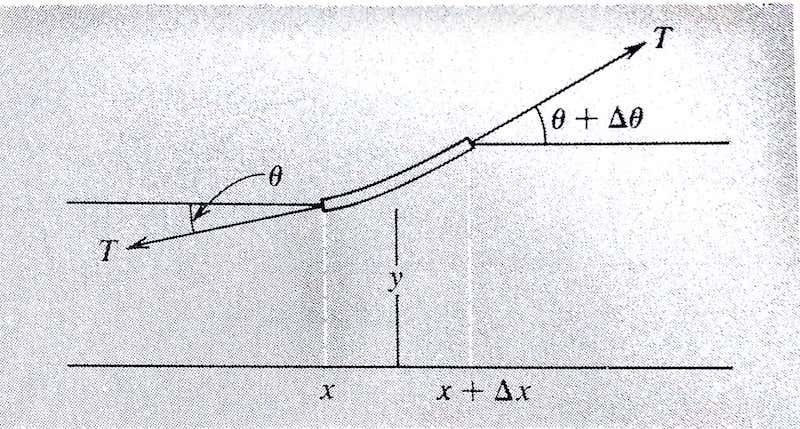
\includegraphics[width=0.85\textwidth]{StringFixedEnds.jpg}
    \pause
    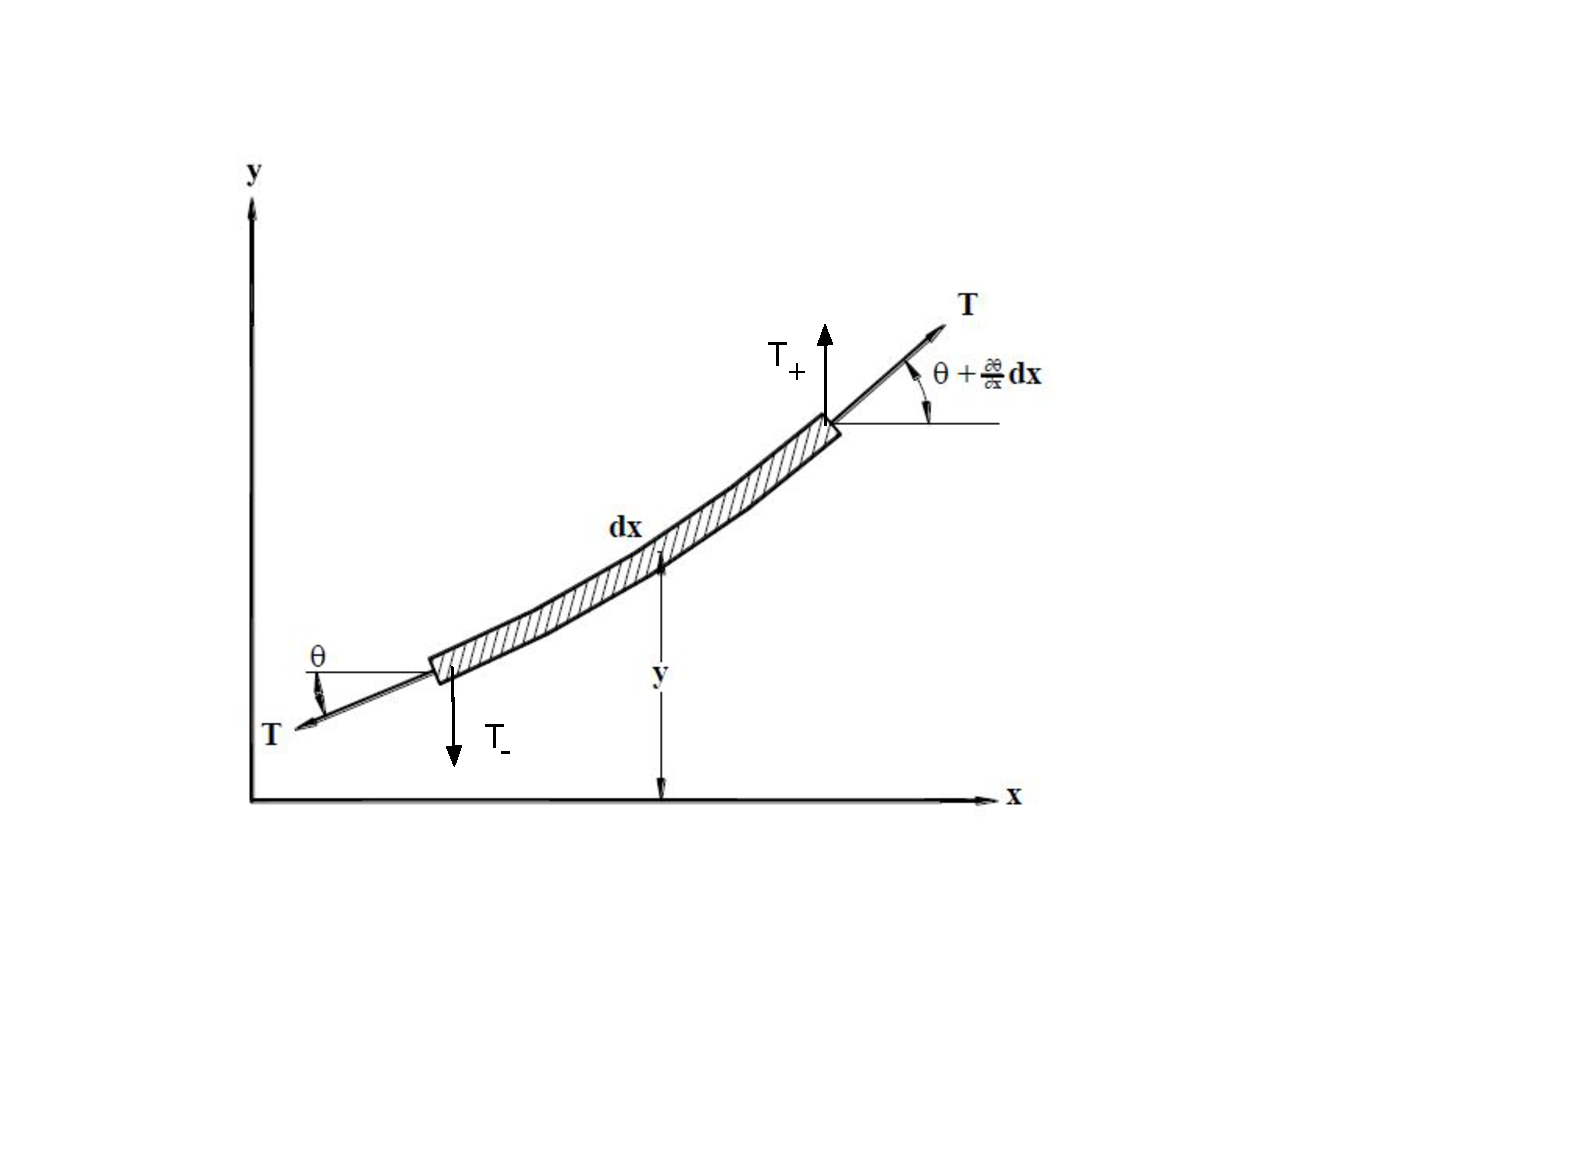
\includegraphics[width=0.85\textwidth]{StringForceDiagram.pdf}
   
each segment has a mass, $m = \mu \Delta x$.
\pause
  \end{column}
  \begin{column}{0.6\textwidth}
    \begin{enumerate}
      \item Small Vibrations ($y << L$)
        \pause
      \item Endpoints are fixed. No displacement $y(0) = y(L) = 0$,
          and no velocity: $\dot{y}(0) = \dot{y}(L) = 0$
        \pause
      \item Constant Tension ($T = \mathrm{const}$). Vibrations are
        small and the changes in string length are $\propto (y/L)^2$
        (negligible). \underline{Magnitude} is constant, but
        \emph{direction} of tension is \textbf{not}.
    \end{enumerate}

  \end{column}
\end{columns}
\end{frame}

\begin{frame}
\frametitle{Analogy with Masses/Springs}
\begin{columns}
  \begin{column}{0.5\textwidth}
    \centering
    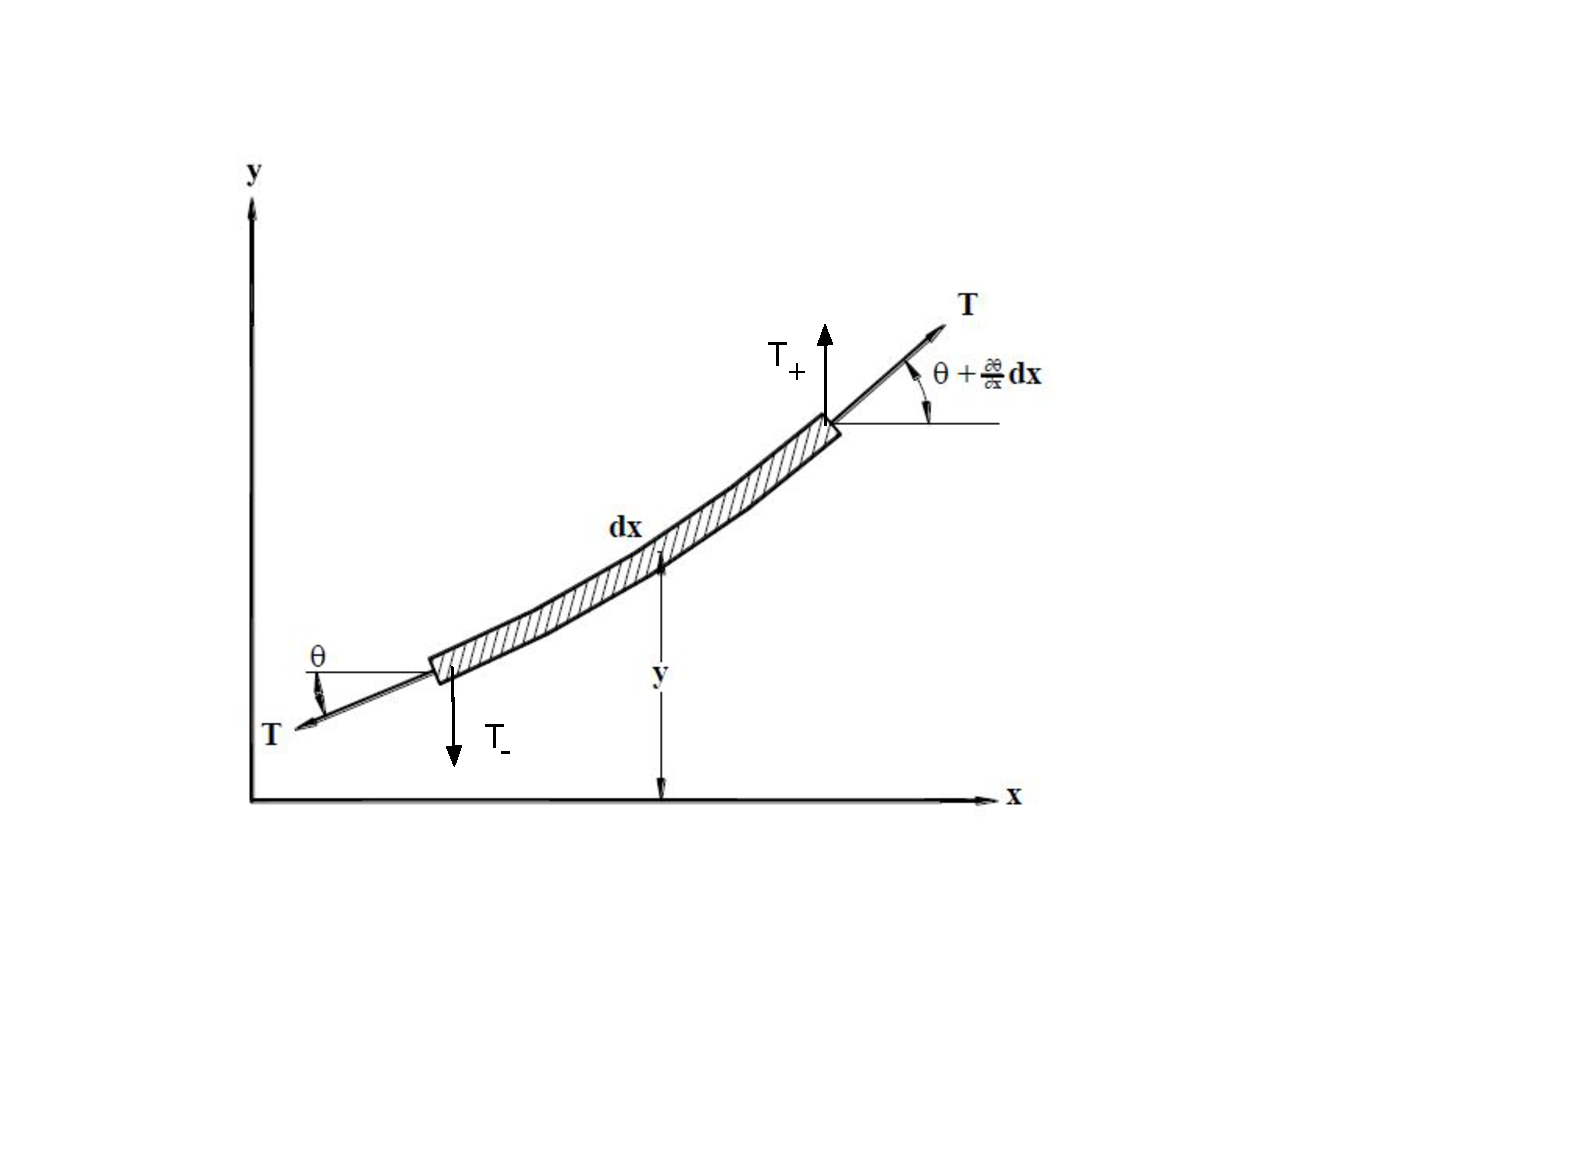
\includegraphics[width=0.75\textwidth]{StringForceDiagram.pdf}
\pause
    \begin{align*}
      \action<+->{m \ddot{y}_p &= T_+ - T_- \\}
          \action<+->{&\simeq T \theta_+ - T \theta_- \\}
    \action<+->{&\simeq T \Bigg[\frac{y_{p+1}-y_{p}}{\Delta x} -
      \frac{y_{p}-y_{p-1}}{\Delta x}\Bigg] \\}
\action<+->{\ddot{y}_p &= \frac{T}{\mu (\Delta x)^2} (y_{p+1} -2 y_p + y_{p-1})}
    \end{align*}


  \end{column}

\begin{column}{0.5\textwidth}
    \centering
    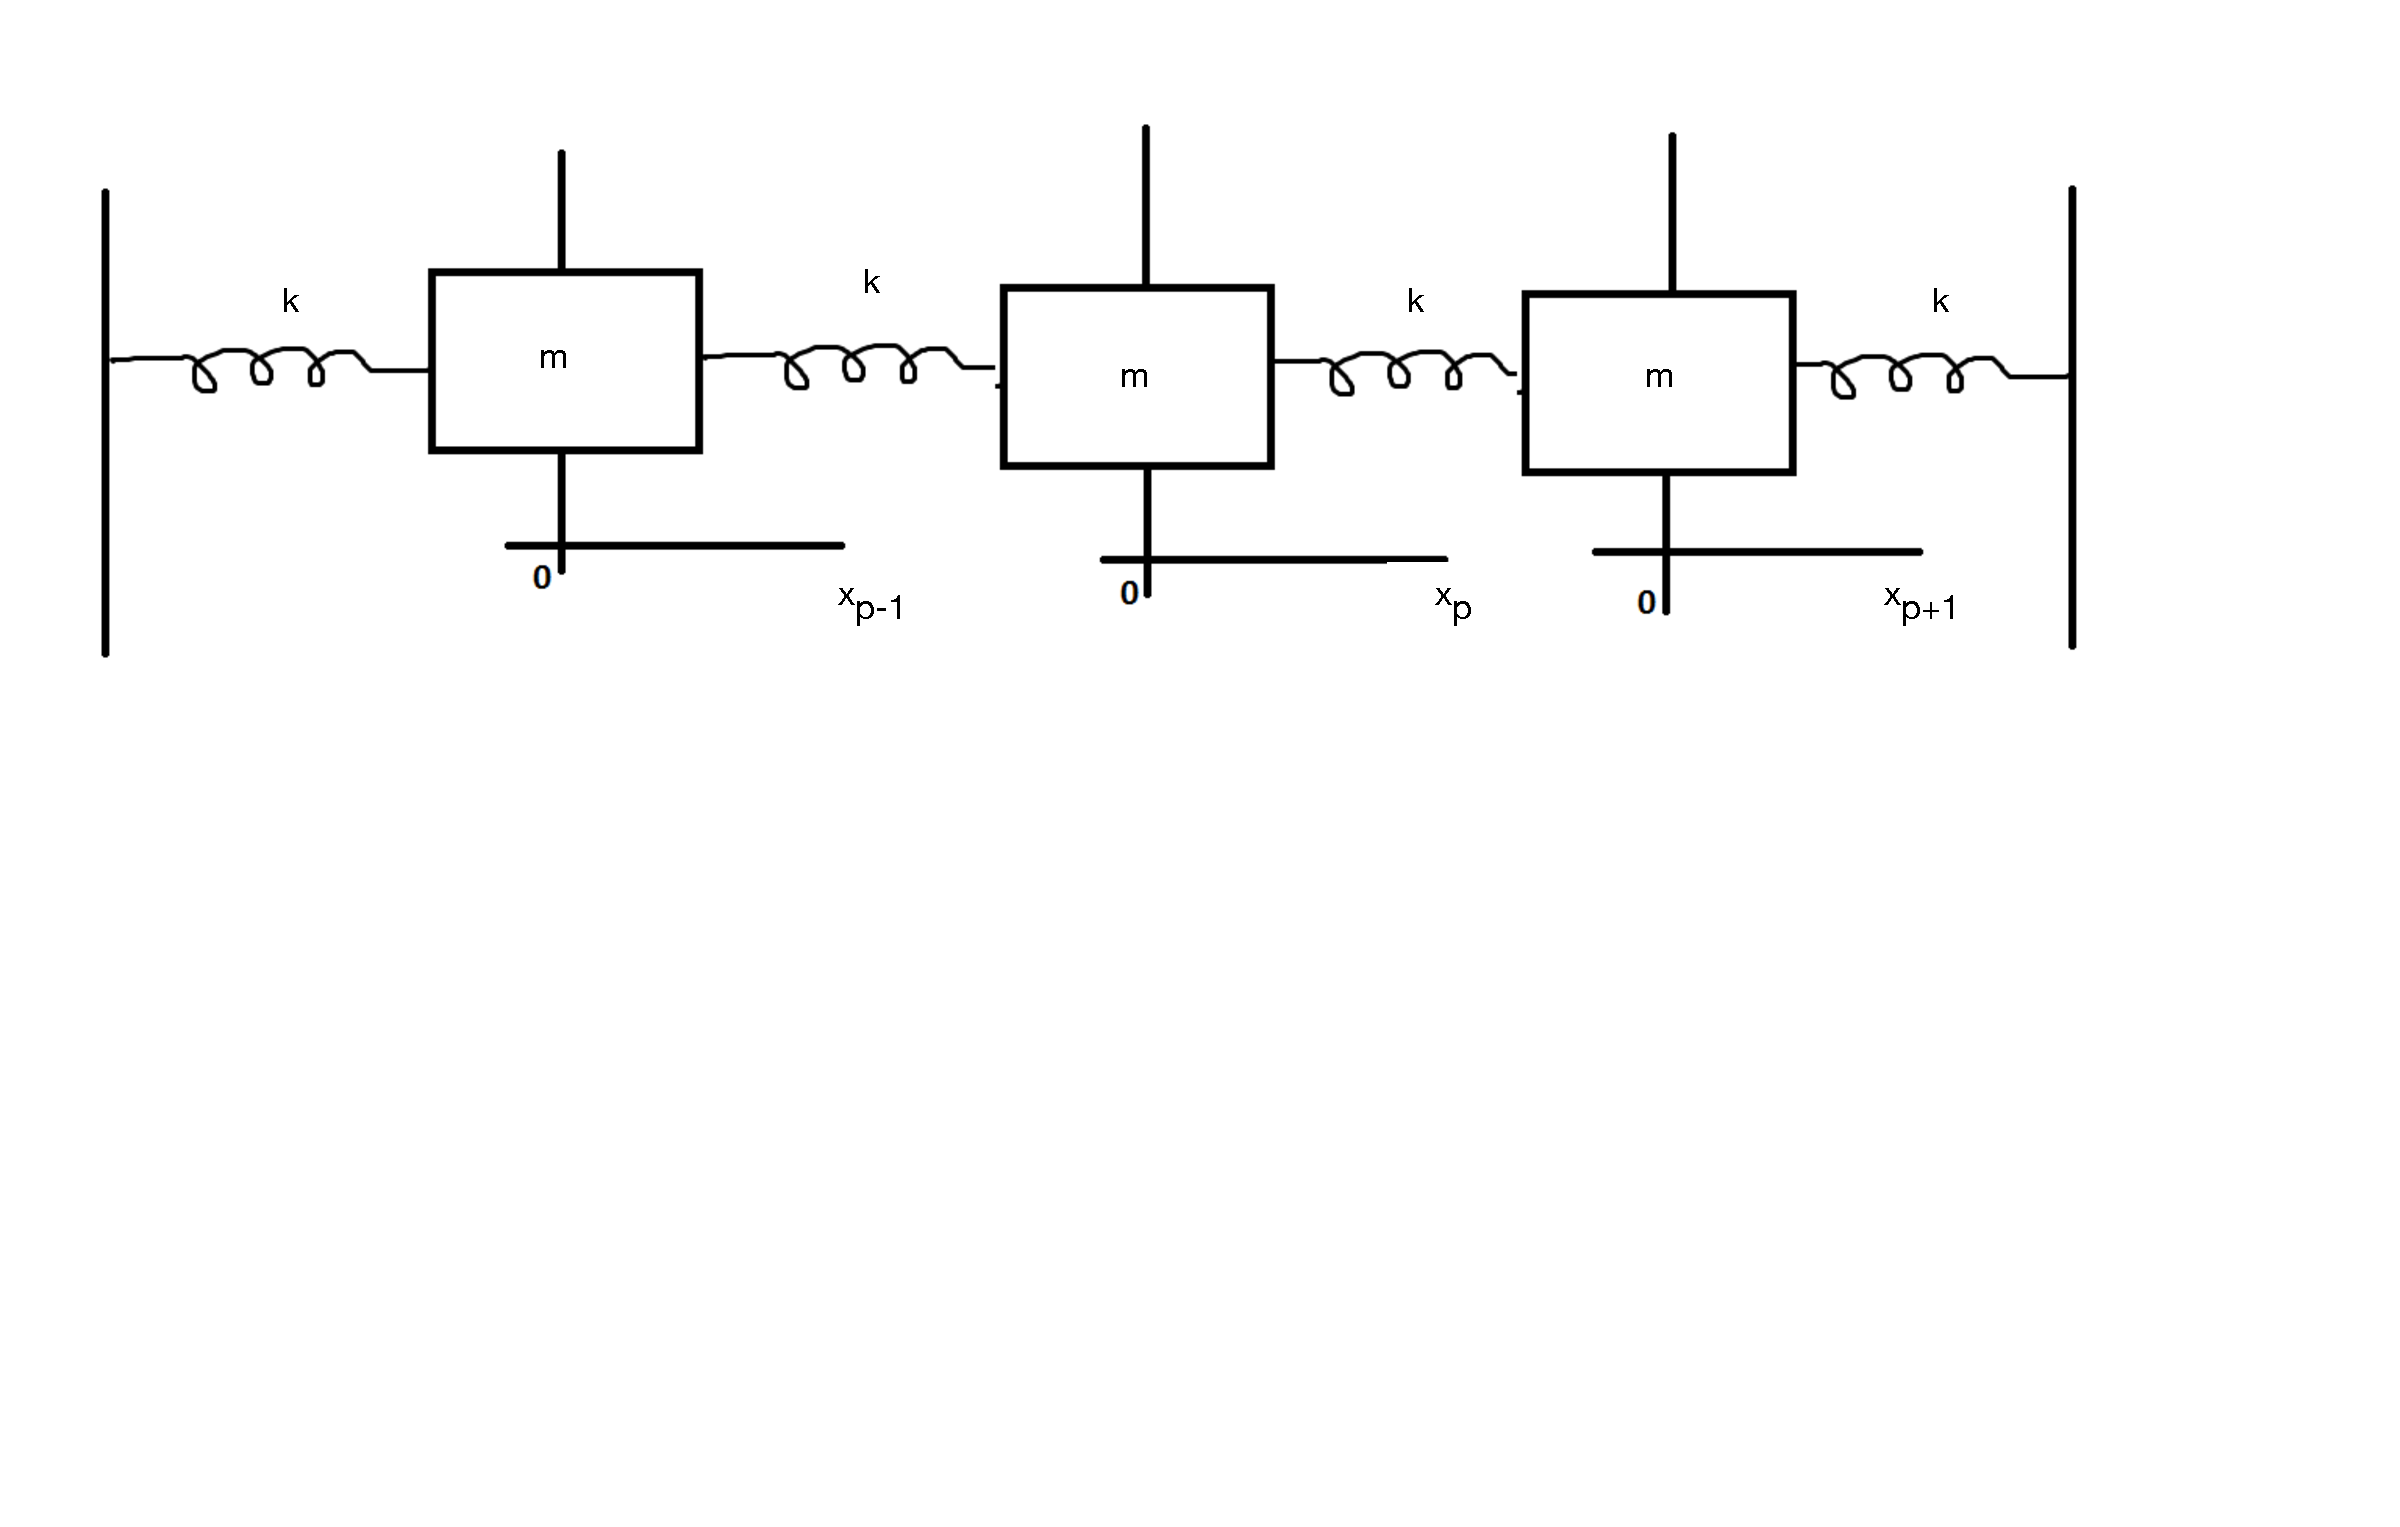
\includegraphics[width=\textwidth]{3mass4spring.pdf}
    \pause
    \begin{align*}
      m \ddot{x}_p &= F_+ - F_- \\
                   &= k (x_{p + 1} - x_{p}) - k (x_{p} - x_{p-1}) \\
      \\
      \\
      \\
      \\
      \\
        \ddot{x}_p &= \omega_0^2 (x_{p+1} - 2 x_p + x_{p-1})  
    \end{align*}

  \end{column}
\end{columns}
\end{frame}


\begin{frame}
\frametitle{Details of the forces / tensions:}
\begin{columns}

  \begin{column}{0.4\textwidth}
    \centering
    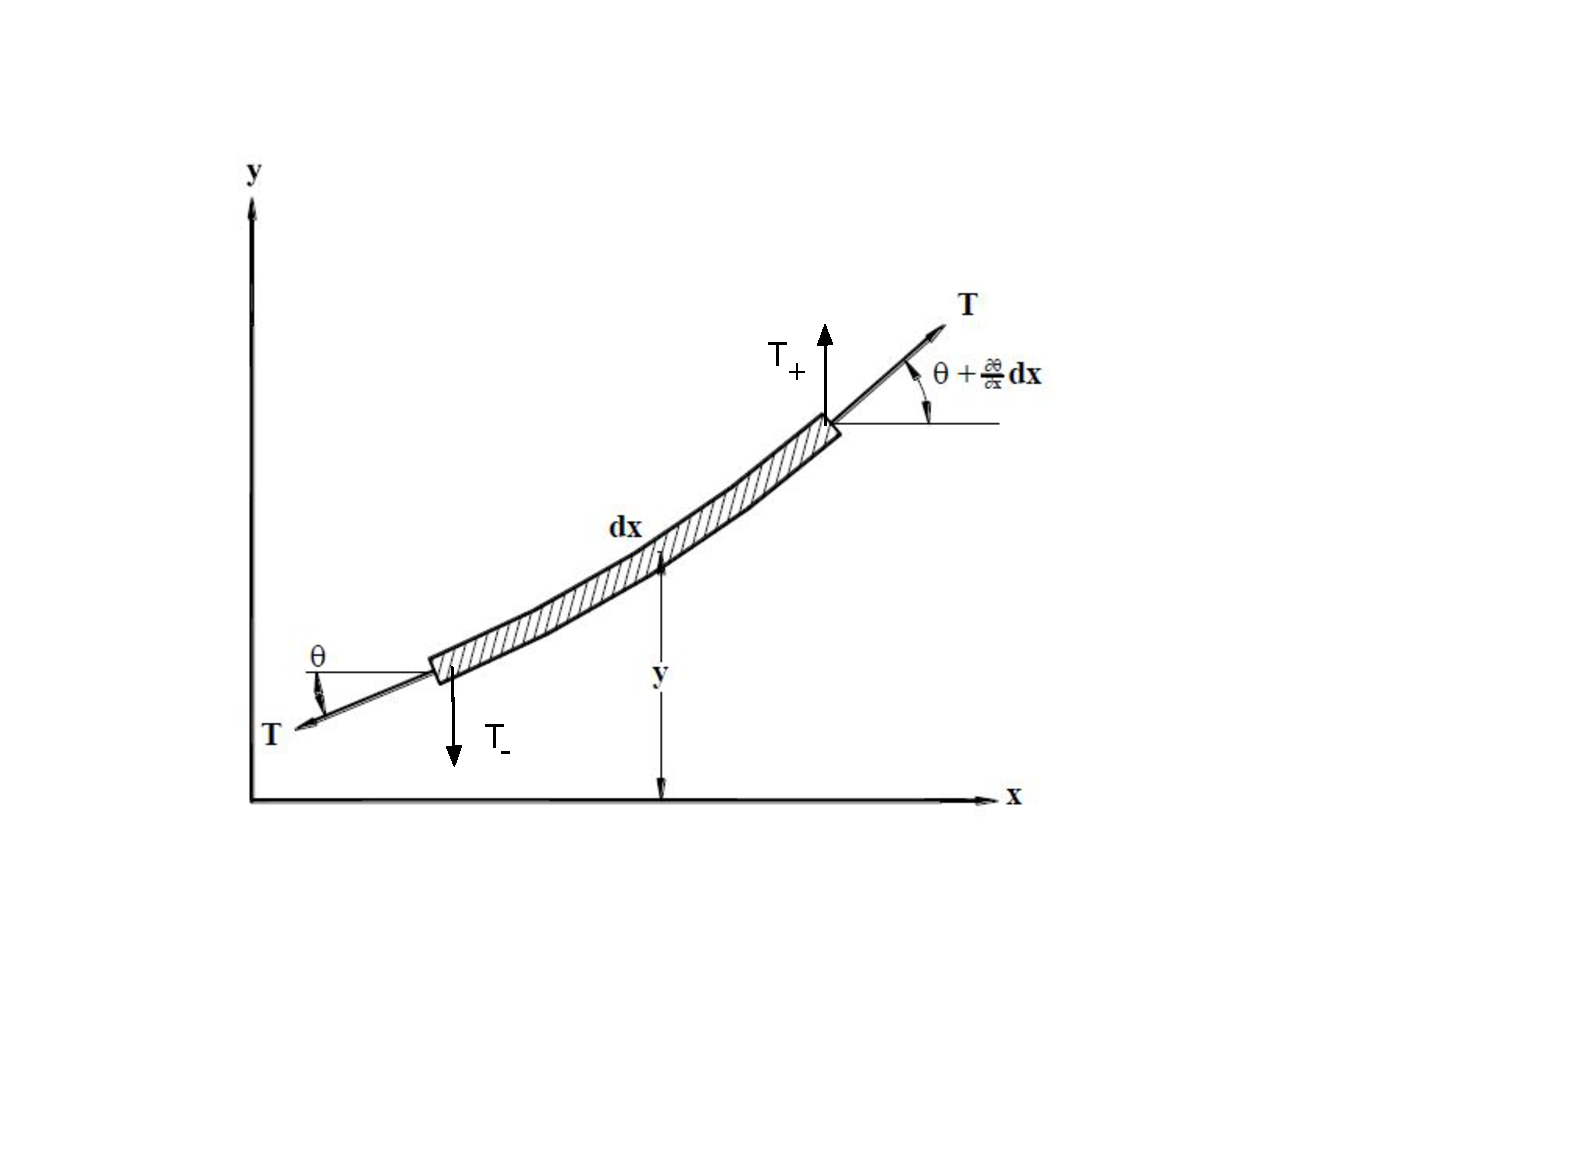
\includegraphics[width=0.85\textwidth]{StringForceDiagram.pdf}

  \end{column}

  \begin{column}{0.6\textwidth}
    \begin{enumerate}
    \item We want to find $y(x,t)$. So far we have:
      \pause
    \item $\ddot{y}_p = \frac{T}{\mu} \frac{\Delta \theta}{\Delta x}$
      \pause
    \item $\frac{\Delta \theta}{\Delta x} = \frac{\theta(x + \Delta x) -
        \theta{x}}{\Delta x}$
      \pause
    \item Small vibrations, so $\theta << 1 \implies$ 
      \pause
    \item $tan(\theta) \simeq \theta \implies$
      \pause
    \item $\theta \simeq \frac{\partial y}{\partial x}$
      \pause
      \item $\frac{\Delta \theta}{\Delta x} = \frac{\partial^2 y}{\partial x^2}$

    \end{enumerate}
  \end{column}
\pause
\end{columns}
So, now we have a relation between time and space:
\pause
\begin{block}{The Wave Equation}
\centering
$ \frac{\partial^2 y}{\partial t^2} = \frac{T}{\mu} \frac{\partial^2 y}{\partial x^2}$
\end{block}


\end{frame}



\section{Wave Equation: Solutions}
\begin{frame}
\frametitle{Wave Equation: Solutions}
\textbf{Technique: Separation of Variables}
\begin{enumerate}
\pause
\item write $y(x,t) = f(x) g(t)$; assumes functions \emph{are} separable
\pause
\item insert into the P.D.E.
\pause
\item P.D.E. $\implies$ ODE for x, ODE for t
\pause
\item impose boundary conditions (e.g. fixed ends, or driven end)
\pause
\item General Solution is sum of these restricted solutions
\end{enumerate}
\end{frame}


\begin{frame}
\frametitle{Wave Equation: Solutions}
\begin{enumerate}
\item $y(x,t) = f(x) g(t)$
\pause
\item 
\begin{align*}
\action<+->{\frac{\partial^2 y}{\partial t^2} &= \frac{T}{\mu} \frac{\partial^2
                                    y}{\partial x^2} \\}
\action<+->{f(x) \frac{\partial^2 g}{\partial t^2} &= v^2 g(t) \frac{\partial^2
                                         f}{\partial x^2} \\}
\action<+->{\frac{1}{g(t)} \frac{\partial^2 g}{\partial t^2} &=
  v^2 \frac{1}{f(x)} \frac{\partial^2 f}{\partial x^2}}
\end{align*}

\pause
\item Since LHS is a function of time \emph{only} and the RHS is a
  function of space \emph{only}, both sides must be equal to a
  constant (call it $\mathcal{C}$). The PDE has been converted into a set of two ODEs.
\end{enumerate}
\end{frame}

\begin{frame}
\frametitle{The ODE Solutions}
\begin{alignat}{2}
\frac{d^2 g}{dt^2} &= \omega^2 g  &\quad g(t) &= C_1 cos(\omega t) \\
\frac{d^2 f}{dx^2} &= -\frac{\omega^2}{v^2} f &\quad f(x) &= A cos(k x) + B
sin(k x) 
\end{alignat}
\pause
where the velocity of the wave, $v \equiv \sqrt{\frac{T}{\mu}}$,
$\frac{\omega}{2 \pi}$ is the frequency, and $k \equiv \omega / v$ is
called the 'wave number'. For the wavelength of the wave, we use the
symbol $\lambda \equiv \frac{2 \pi}{k}$.
\end{frame}

\section{Normal Modes}
\begin{frame}
\frametitle{Normal Modes of a String}
\pause
Let's apply some boundary conditions ! \\
\pause
\begin{enumerate}
\item $f(x) = 0$ for $x \in \{0, L\} \implies$ \\
\pause
\item $sin(k L) = 0$ for any and all t,\\
\pause
\item so $k_n L = n \pi$ or $k_n = n \frac{\pi}{L}$ \\
\pause
\item and $y(x, t) = A_n cos(\omega_n t) sin(k_n x)$ \\
\end{enumerate}

\end{frame}

\begin{frame}
\frametitle{Normal Modes of a String}
\begin{columns}
\begin{column}{0.5\textwidth}

\begin{itemize}
\item Wavelength:  $\lambda_n = \frac{2 L}{n}$

\item Frequency:  $f_n = \frac{v}{\lambda_n}$

\item Velocity:  $v = \sqrt{\frac{T}{\mu}}$

\item $f_n = \frac{n}{2 L} \sqrt{\frac{T}{\mu}}$
\end{itemize}

\end{column}

\begin{column}{0.5\textwidth}

\centering
\includegraphics[width=0.5\textwidth]{stationary-waves-7-638.jpg}

\end{column}
\end{columns}
\end{frame}

\section{Summary}
\begin{frame}
\frametitle{Summary}
\begin{enumerate}

\item Matrix methods can be used to analyzed eigenmodes of linear systems.

\item The case of $N$ springs and $N$ masses can be analyzed as a
  straightforward extension of the methods used for $N = 2, 3$.

\item Strings are an extension of this method to $N \rightarrow \infty$.

\item The Bode plot for systems with finite $N$, and then 
infinite $N$, illustrates the phenomena of \emph{dispersion} and the
\emph{cut-off} frequency.

\item HWK: QP-1, Ch. 5: 6, 10, 11 are coupled oscillator
  problems. 5-16 is for N coupled oscillators; similar to the string problems.

\end{enumerate}
\end{frame}

\end{document}

